\chapter{Binary Collatz Tree}
\label{ch:binary_tree}

\section{Some essentials on binary trees}
A binary tree is a rooted tree, where each node has at most two immediate successors. Those nodes, from which no edge goes out downward, are called leaves, the others are called internal nodes. In a full binary tree, all internal nodes have exactly two children \cite[p.~102]{Ref_Higham_2015}. Full binary trees have an odd number $2n+1$ of nodes. Of these $n+1$ are leaves and $n$ are inner nodes \cite[p.~134]{Ref_Kersting_Wakolbinger_2008}. Each node in a binary tree has a left subtree and a right subtree, which is why a binary tree is inherently recursive, since the left and right subtrees of the root are themselves binary trees \cite[p.~246-247]{Ref_Mazur_2010}. As it often pops up in combinatorial problems, the famous $n$-th Catalan number, named after the Belgian mathematician Eugène Catalan, comes in connection with binary trees into play. For $n\ge1$ it specifies the number of binary trees on $n$ vertices \cite[p.~247]{Ref_Mazur_2010}:
\[
B_n=\sum_{i=0}^{n-1}B_iB_{n-1-i}=\sum_{i=1}^{n}B_{i-1}B_{n-i}=\frac{1}{n+1}\binom{2n}{n}
\]

There is an interesting property that trees exhibit regarding abstract algebra. Let's have a look at the algebraic structure of magmas. Consider an element $x$ of a magma $(M,*)$ which is an iterated product of other elements in $M$. Such an element can be described by a planar (no edges cross each other) rooted binary tree whose $n$ leaves are labelled by these other elements $x_1,\ldots,x_n\in M$ \cite[p.~96]{Ref_Kalka_2016}.

Binary trees make well-suited data structures for storing information. With about $2^m$ data points (nodes), a search of a binary tree takes only about $m$ steps, compared to about $2^{m-1}$ steps which are required to search a simple list \cite[p.~84]{Ref_Benjamin_2009}.

\section{Transforming the Collatz tree into a binary tree}
Jan Kleinnijenhuis and Alissa M. Kleinnijenhuis \cite{Ref_Kleinnijenhuis_2020a} introduced a binary tree $T_{\ge0}$ by transforming the original Collatz tree $H_U$ into the Syracuse tree $H_{C,3}$, which in turn is transformed into the binary tree $T_{\ge0}$ as described next. The edges are changed according to the following procedure: whenever a parent node $w$ has edges to its child nodes $v_0,v_1,\ldots,v_n$, on the tree $H_{C,3}$, we draw an edge from $w$ to $v_0$, and edges from $v_i$ to $v_{i+1}$ for each $i=1,\ldots,n-1$, in the binary new tree. Note that the nodes $v_1,v_2,\ldots,v_n$ are sorted in increasing order of label $v_0<v_1<\ldots<v_n$, which is already given by \ref{eq:n_fold_right_sibling_k}. Figure~\ref{fig:bt3} and \ref{fig:bt3_rot} display that tree -- once in our standard layout and once reversed (from bottom to top).

\begin{figure}[H]
	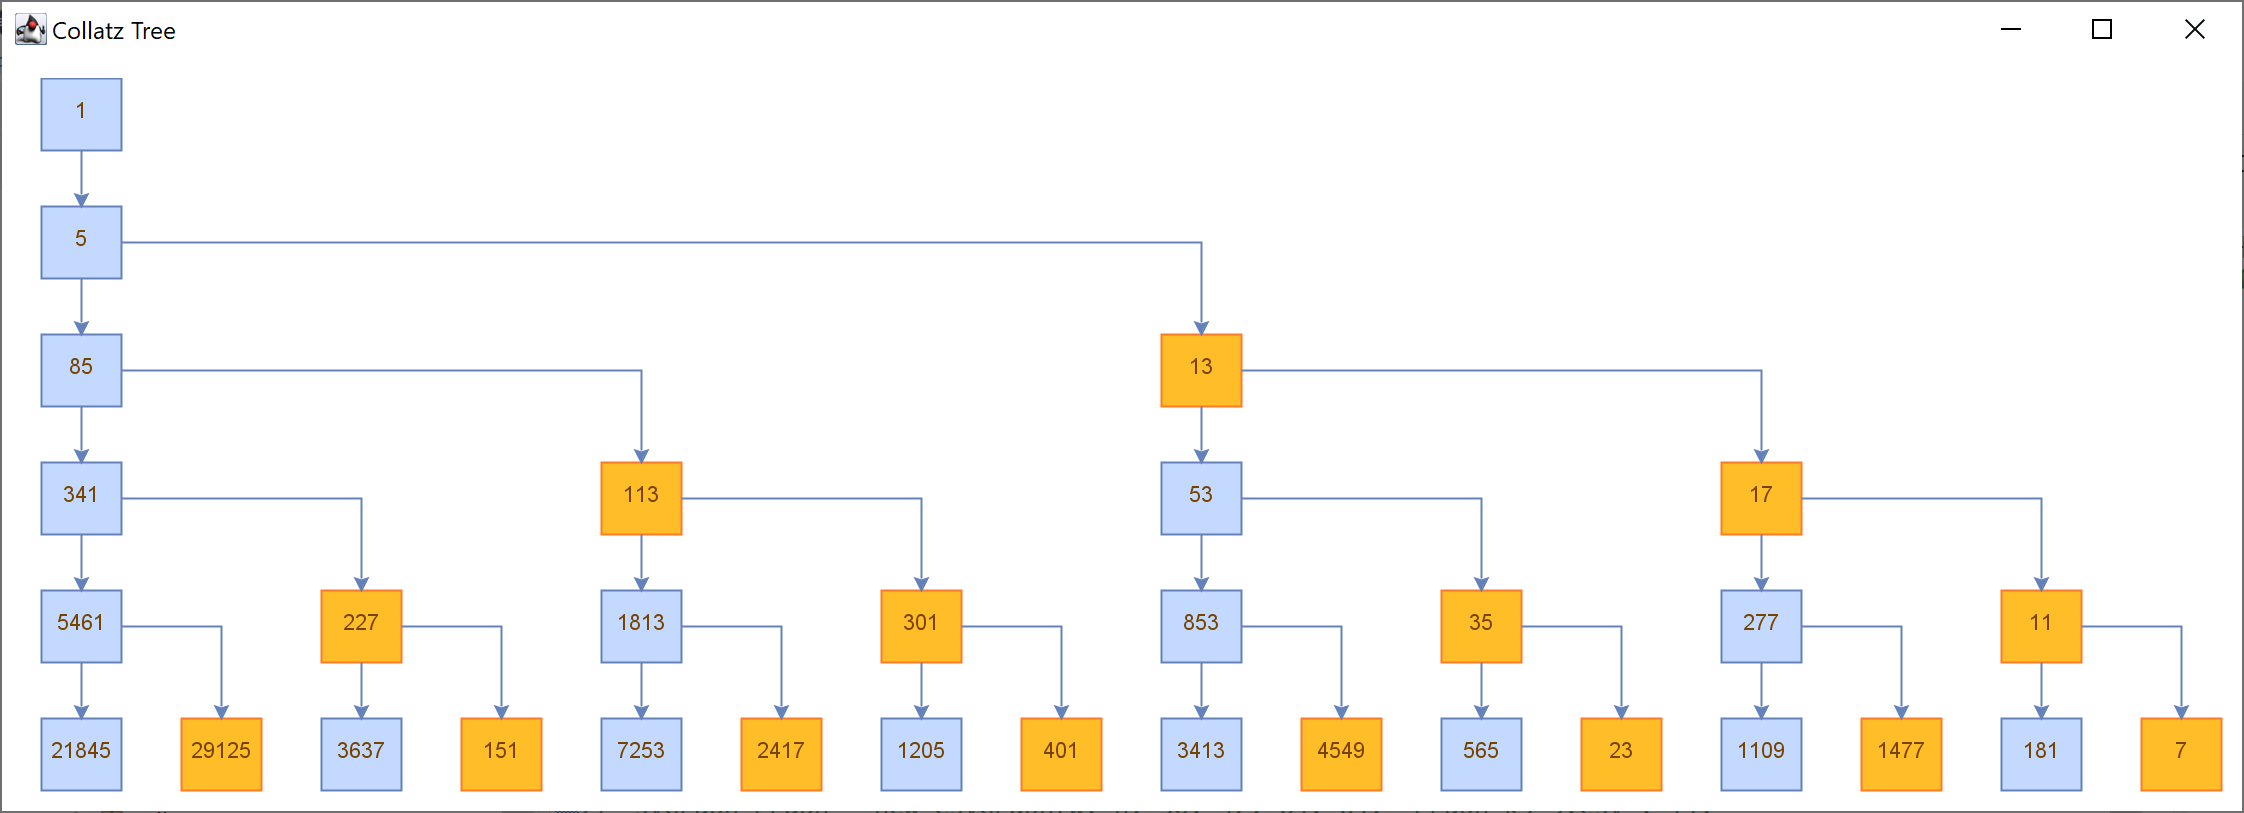
\includegraphics[width=1.00\textwidth]{figures/bt_3_t0.png}
	\caption{The Collatz Tree transformed to the binary tree $T_{\ge0}$}
	\label{fig:bt3}
\end{figure}

\vspace{-2em}
\begin{figure}[H]
	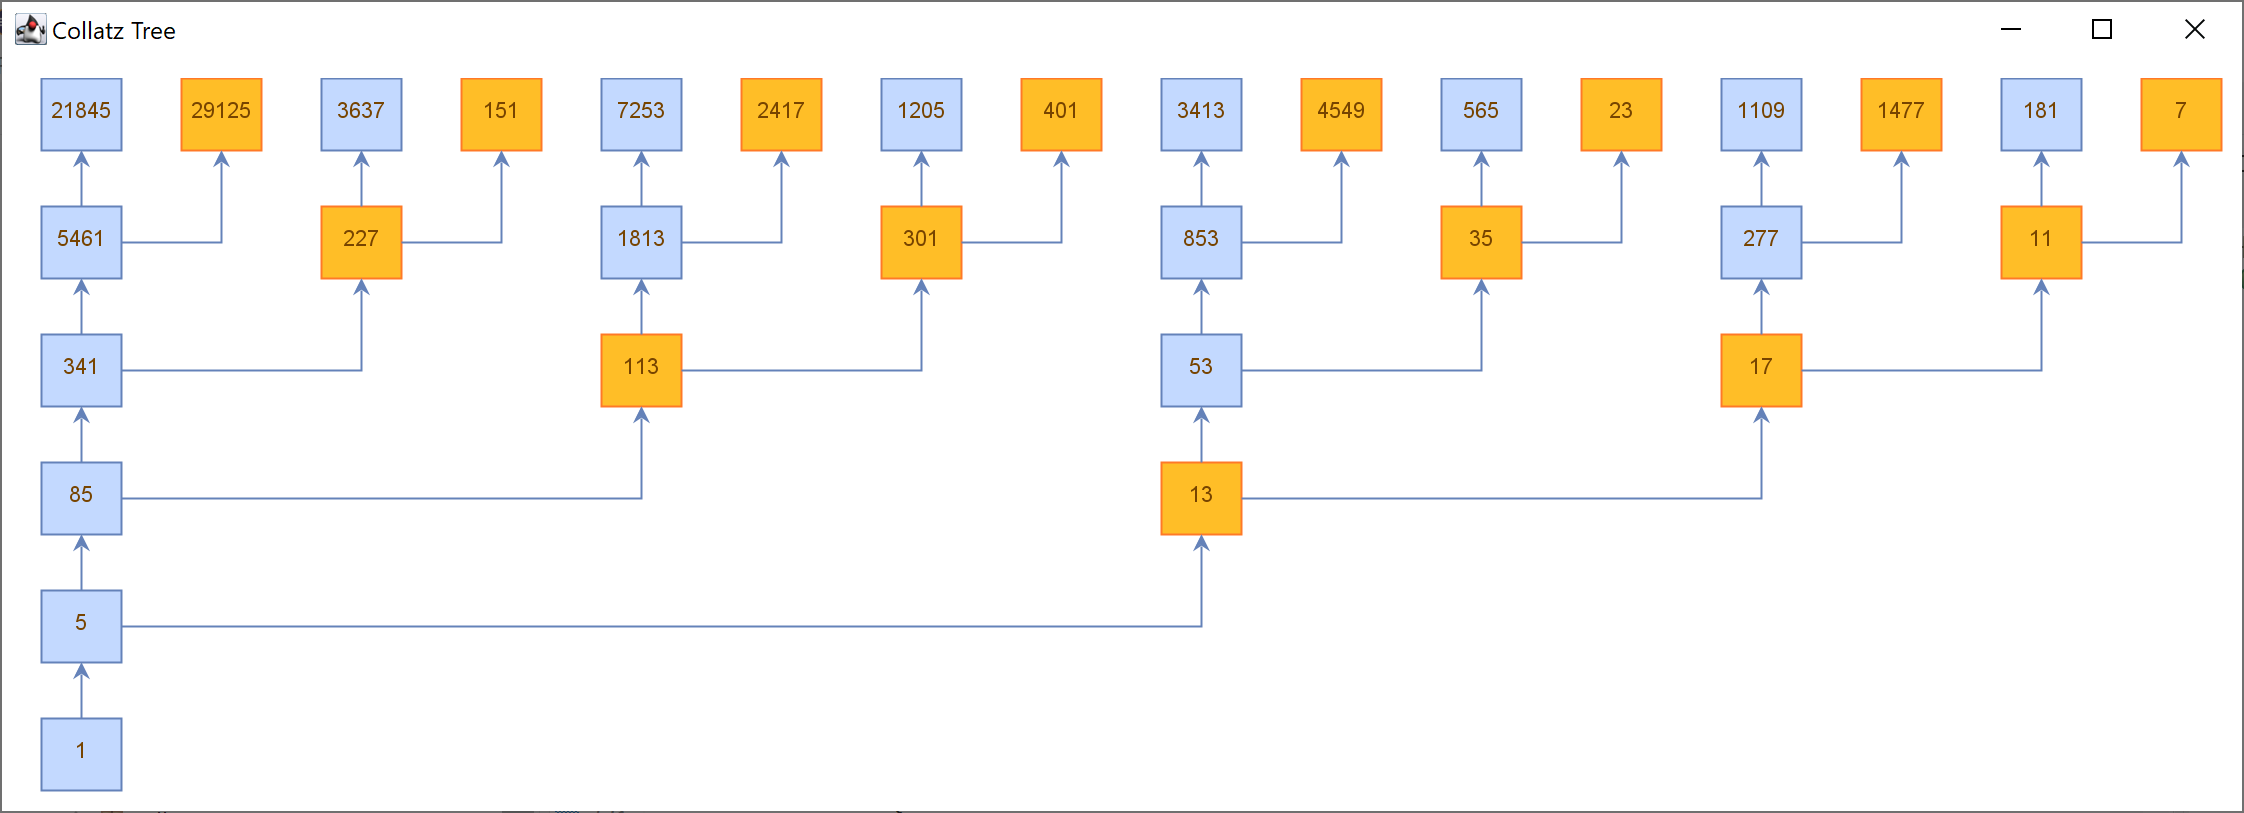
\includegraphics[width=1.00\textwidth]{figures/bt_3_t0_rot.png}
	\caption{The binary tree $T_{\ge0}$ with \textit{bottom-to-top} layout orientation}
	\label{fig:bt3_rot}
\end{figure}

\begin{remark}
	To clarify the terminology, it should be mentioned that Jan and Alissa M. Kleinnijenhuis in their manuscripts \cite{Ref_Kleinnijenhuis_2020a}, \cite{Ref_Kleinnijenhuis_2020b} denote the original Collatz tree $T_C$ while we call it $H_U$. They denote the Syracuse Tree $T_T$ which in our nomenclature is referred to as $H_{C,3}$.
\end{remark}

Nodes that are highlighted orange in figures~\ref{fig:bt3},~\ref{fig:bt3_rot} are called \textit{prunable} and they are exactly those nodes resulting as output of the \textit{Rightward} function. For navigating within this binary tree, Jan Kleinnijenhuis and Alissa M. Kleinnijenhuis \cite{Ref_Kleinnijenhuis_2020a} defined an \textit{Upward} function $U(n)$ and a \textit{Rightward} function $R(n)$ as follows:

\begin{equation}
\label{eq:bintree_3_rightward_upward}
\setlength{\arraycolsep}{1.6em}
\begin{array}{cc}
U(n)=\begin{cases}
        4n+1	&	n\equiv 1\pmod 6\\
        16n+5	&	n\equiv 5\pmod 6
    \end{cases} &
R(n)=\begin{cases}
    \nicefrac{(2^2n-1)}{3}	&	n\equiv 1\pmod{18}\\
    \nicefrac{(2^3n-1)}{3}	&	n\equiv 5\pmod{18}\\
    \nicefrac{(2^4n-1)}{3}	&	n\equiv 7\pmod{18}\\
    \nicefrac{(2^1n-1)}{3}	&	n\equiv 11\pmod{18}\\
    \nicefrac{(2^2n-1)}{3}	&	n\equiv 13\pmod{18}\\
    \nicefrac{(2^1n-1)}{3}	&	n\equiv 17\pmod{18}
\end{cases}
\end{array}
\end{equation}

The domain and codomain of both functions consist of the two residue classes $[1]_6,[5]_6$, which form the multiplicative (cyclic) group $\mathbb{Z}^\ast_6=\{1,5\}=<5>$. Consequently, the domain and codomain exclude all integers divisible by $2$ and $3$, which is due to the fact that this binary tree (just like our tree $H_{C,3}$) does not contain even numbers and additionally all leaves -- namely those nodes labeled with an integer divisible by three -- were deleted. The function $U(n)$ is very similar to the function~\ref{eq:next_sibling_k3} and to the more general function~\ref{eq:n_fold_right_sibling_k} (when setting $n=1,k=3$) which both calculate the right-sibling of a given vertex. This is clear, since siblings (parallel) in $H_{C,3}$ are successors (serial) in the binary tree $T_{\ge0}$. In the end, for a node $v_0$ having a leaf as right-sibling in $H_{C,3}$, the function $U(v_0)$ is defined as $v_1=4v_0+1$ executed twice $v_1=4(4v_0+1)+1=16v_0+5$, because we must skip this leaf. Recall that all leafs in $H_{C,3}$ are excluded from the binary tree without exception. For any $n\in[5]_6$ it applies that $U(n)\equiv16n+5\equiv\boldsymbol{1}\bmod(6)$ since $6\mid16n+5-\boldsymbol{1}$ resulting in $6\mid16(5+k\cdot6)+5-\boldsymbol{1}$, see \ref{eq:congruence}, and analogously for any $n\in[1]_6$ it applies that $U(n)\equiv4n+1\equiv\boldsymbol{5}\bmod(6)$ since $6\mid4n+1-\boldsymbol{5}$ resulting in $6\mid4(1+k\cdot6)+1-\boldsymbol{5}$. Therefore executing the Upward function twice in a row leads unconditionally to $U^2(n)=16(4n+1)+5=4(16n+5)+1=64n+21$.

\begin{remark}
	While we displayed trees from top to down, it is sometimes usual to draw trees in a bottom-to-top fashion as Kleinnijenhuis \cite{Ref_Kleinnijenhuis_2020b} do. The Rightward function corresponds to what we call left-child and the Upward function relates to the right-child which is commonly used in the context of binary trees \cite[p. 246]{Ref_Mazur_2010}.
\end{remark}

Jan and Alissa M. Kleinnijenhuis \cite{Ref_Kleinnijenhuis_2020a} defined the set $N(T_C)=N(H_U)$ that contains the labels of all nodes, to which a path from the root in $H_U$ exists, in other words, this set contains all integers $n$ for which the orbit of $n$ under the (uncompressed) Collatz function~\ref{eq:func_collatz} converges to $1$. Furthermore they introduced $S_{\ge0}$ as the node set containing integers that are neither divisible by $2$ nor by $3$. The set $S_{-1}$ comprises on the contrary all numbers, which are divisible by $2$ or $3$. In order to comprehend the structure of these sets $S$, let us take a look at the following list showing which tree includes which node set, see also the ancillary files of \cite{Ref_Kleinnijenhuis_2020a}, \cite{Ref_Kleinnijenhuis_2020b}:

\[\arraycolsep=0.6em\def\arraystretch{1.4}
\begin{array}{llll}
\text{Original Collatz tree} & N(T_C)=N(H_U)&=&\mathbb{N^+} \hspace{0.6em}\text{if the Collatz conjecture holds}\\
\text{Syracuse tree} & N(T_T)=N(H_{C,3})&=&N(T_C)\setminus2\mathbb{N}\\
\text{Binary tree}\hspace{0.6em}T_{\ge0}& N(T_{\ge0})=S_{\ge0}&=&N(T_C)\setminus S_{-1}\hspace{2.1em}=S_{0}\cup S_{1}\cup S_{2}\ldots\\
\text{Binary tree}\hspace{0.6em}T_{\ge1}& N(T_{\ge1})=S_{\ge1}&=&N(T_C)\setminus \bigcup_{i=-1}^{0}S_i=S_{1}\cup S_{2}\cup S_{3}\ldots\\
\text{Binary tree}\hspace{0.6em}T_{\ge j} & N(T_{\ge j})=S_{\ge j}&=&N(T_C)\setminus \bigcup_{i=-1}^{j-1}S_i=\bigcup_{i=j}^{\infty}S_i
\end{array}
\]

\par\medskip
Let us describe these sets using multiplicative groups. The set $S_{\ge0}=\mathbb{Z}^\ast_6$ can be understood as the multiplicative group modulo $6$ and the set $S_{-1}=\mathbb{Z}/6\mathbb{Z}\setminus\mathbb{Z}^\ast_6=\{0,2,3,4\}$ as the set of all non-invertible elements (non-units) of $\mathbb{Z}/6\mathbb{Z}$.

The set $S_0$ consists of all nodes resulting as output of $R(n)$ within the binary tree $T_{\ge0}$. These are the orange highlighted nodes displayed by figures~\ref{fig:bt3},~\ref{fig:bt3_rot}. In other words, $S_0$ is the codomain of the function $R(n)$ operating on nodes within $T_{\ge0}$. The binary tree $T_{\ge0}$ can be transformed to a (pruned) binary tree $T_{\ge1}$. For this, the prunable nodes will be deleted and their neighbors reconnected. The upward neighbor of a pruned node will then be identified as pruning candidate for a later transformation of the resulting tree $T_{\ge1}$ to a more pruned tree $T_{\ge2}$.

The set $S_1$ contains all nodes that are (as per the description above) identified as pruning candidates for the next transformation of $T_{\ge1}$ to $T_{\ge2}$. After having transformed $T_{\ge1}$ to $T_{\ge2}$, the more pruned binary tree $T_{\ge2}$ contains nodes that are identified as pruning candidates for another upcoming transformation of $T_{\ge2}$ to $T_{\ge3}$ -- these nodes are elements of the set $S_2$. This pruning algorithm is repeatedly applied in the same pattern. And in this way we obtain the sets $S_1,S_2,S_3,\ldots$ and so forth. Generally, we can write these sets in the form $S_j=\{n\in N(T_{j-1})\mid U^{-j}(n)\in S_0\}$. Kleinnijenhuis found out that the codomain $\mathbb{N}^U$ of the Upward function contains $5$ residue classes modulo $96$, namely $\{5, 29, 53, 77, 85\}=\mathbb{N}^U$ and the codomain $\mathbb{N}^R$ of the Rightward function comprises $27$ residue classes modulo $96$, namely $\{1, 7, 11, 13, 17, 19, 23, 25, 31, 35, 37, 41, 43, 47, 49, 55, 59, 61, 65, 67, 71, 73, 79, 83, 89, 91, 95\}=\mathbb{N}^R$. The union of both sets $\mathbb{N}^U\cup\mathbb{N}^R$ forms the non-cyclic multiplicative group $\mathbb{Z}^\ast_{96}=<\{5, 17, 31\}>$ (see \cite{Ref_Lang_2017}, \cite{Ref_OESIS_A033949}).

Let us take a closer look at the (cyclic) multiplicative group $\mathbb{Z}^\ast_{18}=\{1,5,7,11,13,17\}=<5>$ which has an order $ord(\mathbb{Z}^\ast_{18})=6$. Having the generator $5$ coprime to the modulus $18$, we obtain the congruence $5^{\phi(18)}\equiv1\pmod{18}$ in accordance with Euler's theorem \ref{eq:eulers_theorem}. This allows us to infer from $5^6\equiv5^{6(n+1)}\equiv5^j5^{6n+6-j}\equiv1\pmod{18}$ the congruences given by \ref{eq:homomorphism_congruences} (on the left).

If $m\mid n$, as in our case $3\mid18$, then the map $f:\mathbb{Z}^\ast_n\rightarrow \mathbb{Z}^\ast_m$ with $f(r\bmod n)=r\bmod m$ is a homomorphism as long as $\gcd(r\bmod n,n)=1$ leads to $\gcd(r\bmod m,m)=1$. By Euclid, we know that in the case $r$ is coprime to $n$ then it is also coprime to every factor $m$ of $n$. That is why a homomorphism exist to the congruences shown in \ref{eq:homomorphism_congruences} (on the right).

\begin{equation}
\label{eq:homomorphism_congruences}
\begin{array}{lllll}
	j=0 & [1]_{18}\cdot5^{6n+6}&\equiv1\pmod{18}&\hspace{4em}[1]_{18}\cdot4 &\equiv1\pmod{3}\\
	j=1 & [5]_{18}\cdot5^{6n+5}&\equiv1\pmod{18}&\hspace{4em}[5]_{18}\cdot8 &\equiv1\pmod{3}\\
	j=2 & [7]_{18}\cdot5^{6n+4}&\equiv1\pmod{18}&\hspace{4em}[7]_{18}\cdot16 &\equiv1\pmod{3}\\
	j=3 & [17]_{18}\cdot5^{6n+3}&\equiv1\pmod{18}&\hspace{4em}[17]_{18}\cdot2 &\equiv1\pmod{3}\\
	j=4 & [13]_{18}\cdot5^{6n+2}&\equiv1\pmod{18}&\hspace{4em}[13]_{18}\cdot4 &\equiv1\pmod{3}\\
	j=5 & [11]_{18}\cdot5^{6n+1}&\equiv1\pmod{18}&\hspace{4em}[11]_{18}\cdot2 &\equiv1\pmod{3}
\end{array}
\end{equation}

\newpage

Figure~\ref{fig:tree_transformations} shows the complete chain of tree transformations, beginning from the original Collatz tree, over the Syracuse tree to the binary tree and pruned ones.

% trim=left bottom right top
\begin{figure}[H]
	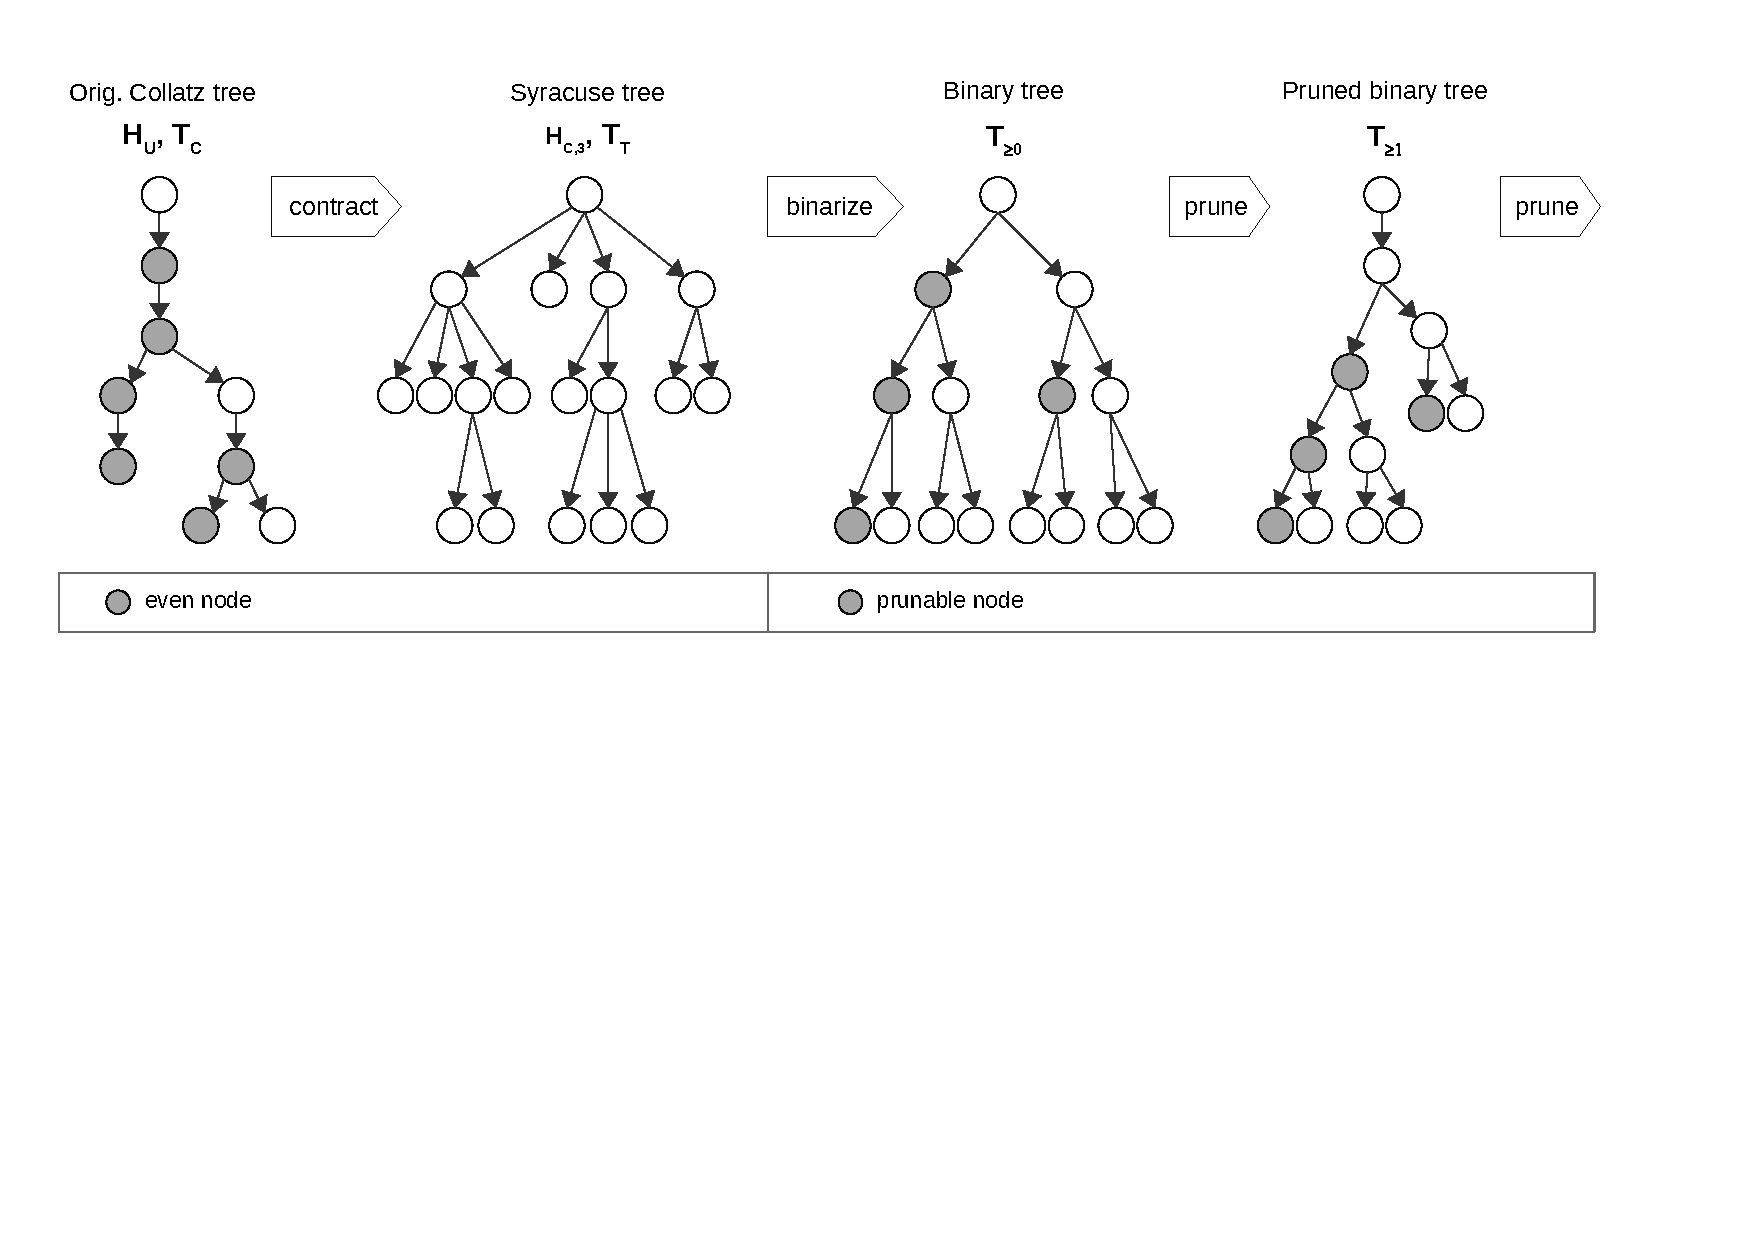
\includegraphics[trim=1.1cm 10cm 2.6cm 0.2cm, 
	width=1.00\textwidth,page=1]{figures/tree_transformations.pdf}
	\caption{Transformation chain, beginning from the original Collatz tree up to pruned binary trees}
	\label{fig:tree_transformations}
\end{figure}